
Like the fully leptonic decay $H\rightarrow WW \rightarrow l^{+}l^{-}\nu\bar{\nu}$, the $H\rightarrow ZZ\rightarrow l^{+}l^{-}\nu\bar{\nu}$  
final state also consists of two isolated leptons and large missing energy from the two undetectable neutrinos. However, the kinematic properties
of these two final states are different. Because in $H\rightarrow ZZ$ both neutrinos originate from $Z$ decay, the amount of missing transverse 
energy depends strongly on the Higgs mass. There is no missing tranverse energy in an event if the $Z$ is produced at rest. Because the
requirement of large \met 
is necessary to supress Drell-Yan background, the analysis is sensitive only to high mass ($m_{H}>250$ \GeVcc) 
Higgs boson production, where the vector bosons are typically boosted. We use the event selections defined in Ref.~\cite{ref:HWW2011smurf}:

Most considerations presented in the previous section apply to the matrix element based method for the $H\rightarrow ZZ$ analysis,
however a few distinct features need to be highlighted. 

In this analysis, for each event  we calculate probabilities for six signal hypotheses (  $H\rightarrow ZZ\rightarrow l^{+}l^{-}\nu\bar{\nu}$
with $m_{H}=$250, 300, 350, 400, 500, and 600 \GeVcc) and for three background hypotheses ($WW$, $WZ$, and $ZZ$). Most of the
$Z$+jets background is removed by the \met requirement, therefore we do not expect a significant performance degradation due to
excluding this process from the matrix element calculations. In the calculation of the $WZ$ probability, we assume that the two reconstructed
charged leptons are originating from a $Z$, and the lepton from the decay of the $W$ boson is not reconstructed. This is a good 
approximation provided that the reconstructed lepton pair is required to have an invariant mass consistent with the $Z$.

Another difference with respect to the $H\rightarrow WW$ analysis, is that here we perform the analysis inclusive in the number of jets. 
However, the $K(k_x,k_y)$ model is extracted from Monte Carlo for each $N_{jets}$ bin (0 jets, 1 jet, and 2 or more jets) separately. 
Figure~\ref{fig:zzboost} shows a comparison of the distributions of transverse boost for gluon fusion Higgs production 
at three different values of $m_H$ and the non-resonant $WZ$ and $ZZ$ processes.

\begin{figure}[!htbp]                                                                                         
\begin{center}                                                                                                
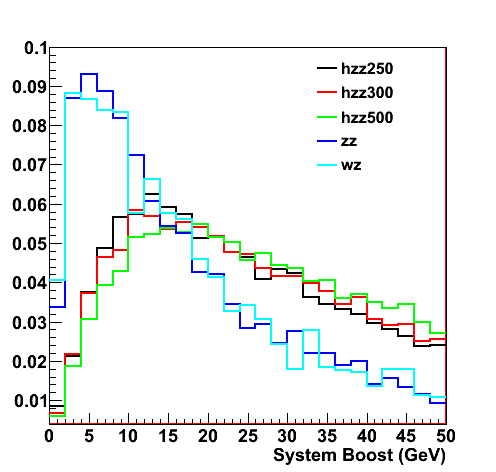
\includegraphics[width=0.5\textwidth]{figures/hzz_boost_allj.png}                                                      
\caption{The transverse boost of the diboson system for $ZZ$, $WZ$ production and $H \rightarrow ZZ$ at 3 different Higgs masses.} 
\label{fig:zzboost}                                                                                           
\end{center}                                                                                                  
\end{figure}  
 
The evaluation of lepton efficiency functions is identical to the method described in Section~\ref{sec:EfficiencyTransfer}, with the 
exception that $ZZ$ Monte Carlo is used instead of $WW$. The transfer function for charged leptons is considered to be a $\delta$-function.
Transverse components of \met are inferred from the lepton momenta and the system boost using tranverse momentum conservation.
The special treatment of fake leptons, described in Section~\ref{sec:FakeLeptons}, is not needed because in the current implementation
the $Z$+jets background is not included into the list of processes for which matrix element based probabilities are calculated. 

Event probabilities, calculated as described above, are used to construct the likelihood ratio discriminant, 
which we use in a one-dimensional template fit.  The discriminator for $H\rightarrow ZZ$ is defined as :
\begin{equation}
\label{eqn:LRHZZ}
LR = \frac { P_{HZZ}} { P_{HZZ} + k_{WW} P_{WW}+ k_{WZ} P_{WZ} + k_{ZZ} P_{ZZ}},
\end{equation}
where $k_{i}$ are the relative ratio of expected contributions of each background and satisfy $\sum k_{i} =1$.
Like $P_{HWW}$, the calculation of $P_{HZZ}$ is a function of Higgs mass so the likelihood ratio shape depends on $m_H$. 
This is true for both signal and background templates of $LR$
